%!TEX root = ../main.tex

\subsection{Geometric component}
\label{ss:geometric_component}

As may have become clear from the previous section, the only available information for the construction of the geometric component (and normal component) are the three vertices that define a single primitive. The vertices contain the vertex \textit{xyz} coordinates together with a unique normal per vertex i.e. the normals of each vertex is the same for every primitive using that vertex. Figure \ref{fig:method:input_primitive} contains an illustration of ``'the input primitive'' for which we will henceforward will omit the explicit reference. 

\begin{figure}
	\centering
	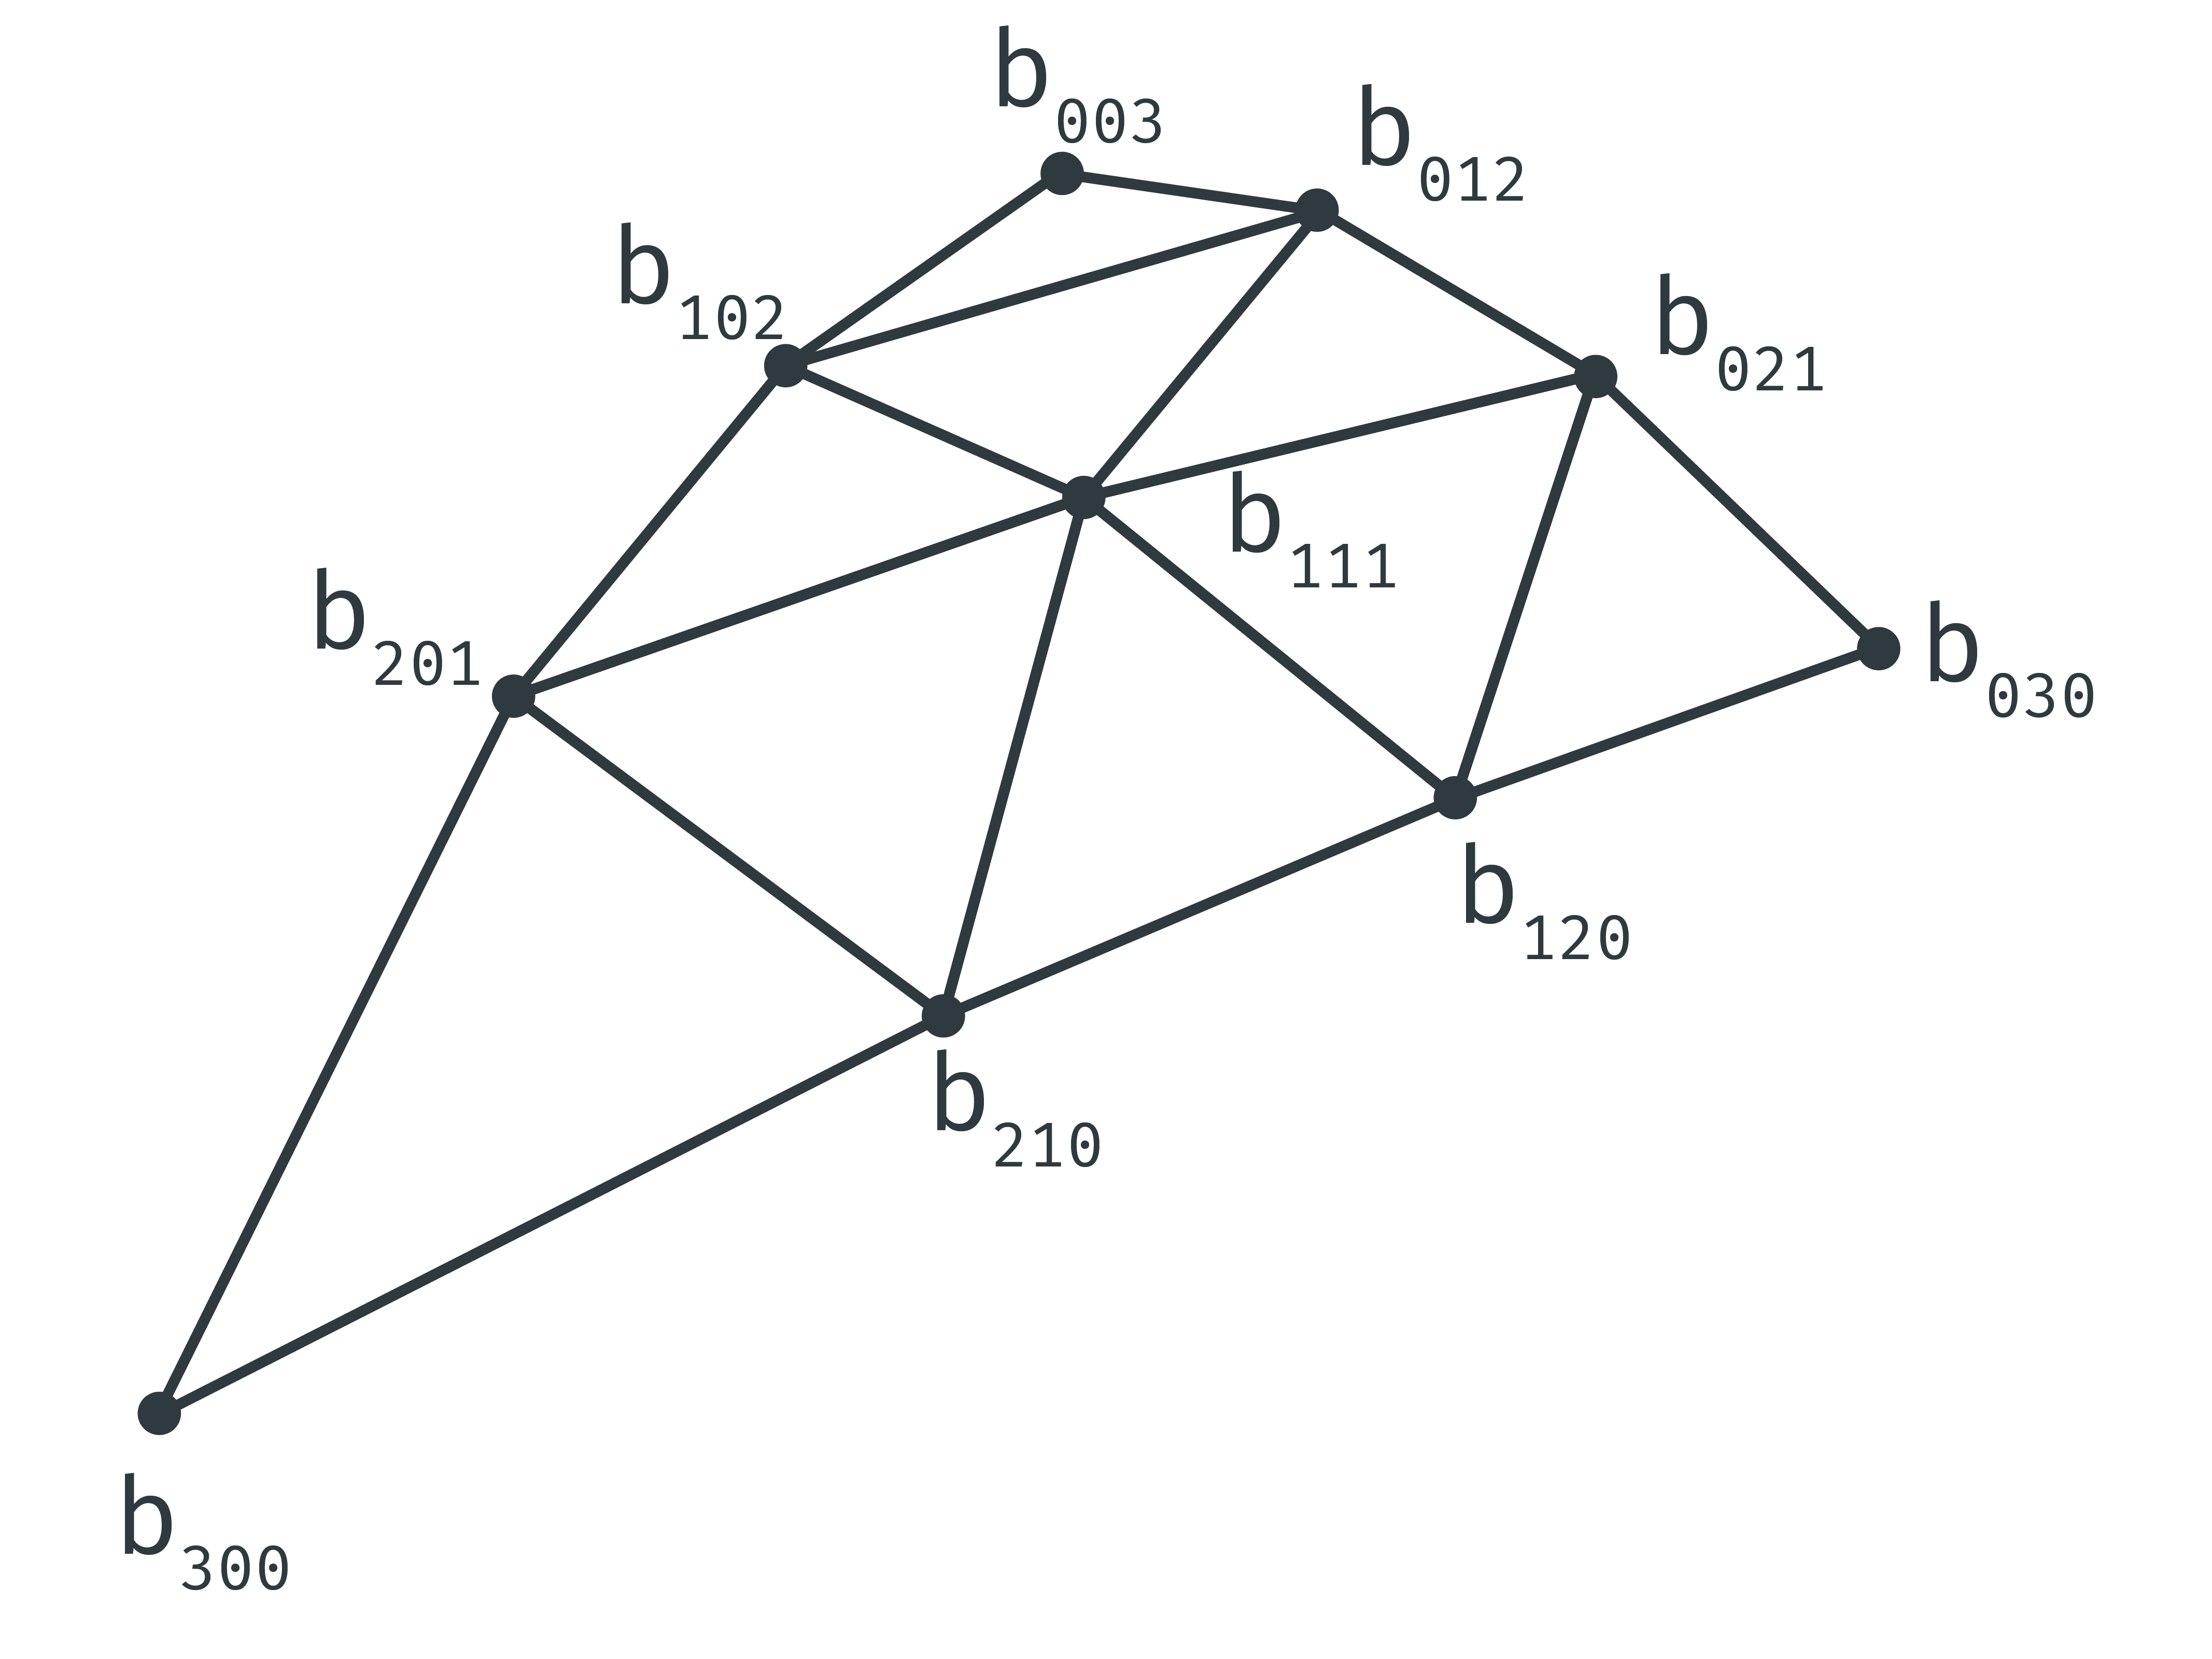
\includegraphics[width=0.45\textwidth]{./content/img/method/geometry.png}
	\caption{The geometric component: the control net of a triangular B\`ezier patch.}
	\label{fig:method:control_net}
\end{figure}

The geometric component of a PN triangle is defined by a triangular cubic B\`ezier patch. In figure \ref{fig:method:control_net} a visualization the network of the coefficients, also know as control points, is shown. A cubic B\`ezier patch $b$ is given by:

\begin{align}
\noalign{$b: \quad R^2 \mapsto R^3,\quad$ for $w = 1 - u - v, \quad u, v, w \geq 0$}
\begin{split}\label{eq:method:cubic_bezier_patch}
    b(u,v) ={}& \sum_{i + j + k = 3} b_{ijk}\frac{3!}{i!j!k!} u^i v^j w^k,\\
      	   ={}& b_{300}w^3 + b_{030}u^3 + b_{003}v^3\\
      	    {}& + b_{210}3w^3 + b_{120}3wu^2 + b_{201}3w^2v\\
      	    {}& + b_{021}3u^2v + b_{102}2wv^2 + b_{012}3uv^2\\
      	    {}& + b_{111}6wuv.
\end{split}
\end{align}

The control points are grouped together (see figure \ref{fig:method:control_net}) as follow:

\begin{itemize}\label{eq:method:control_coefficients}
	\item [vertex coefficients:]  $b_{300},\ b_{030},\ b_{003}$\\
	% \text{tangent coefficients: } {}& b_{210},\ b_{120},\ b_{021},\ b_{012},\ b_{102},\ b_{201} \\
	% \text{center coefficient: }   {}& b_{111}\nonumber\\
\end{itemize}

\todo[inline]{We express geometric compinent as a cubic patch}
\todo[inline]{Discuss parametrization of cubic patch}
\todo[inline]{Discuss the construction of the control points for the cubic patch}